\chapter{Reduction to the assignment problem}

\section{Introduction}
In this chapter, we will show how we can reduce the problem of finding the optimal partition of the nodes of a tree $T$ given their equivalence classes into $p$ with $p \leq |E| \leq t$ chains to the Minimum Weight Perfect Bipartite Matching problem, where $E$ is the set of equivalence classes of the nodes of $T$ and $t$ is the number of nodes of the tree. This reduction will allow us to solve the problem in polynomial time as shown in the previous chapter.

Then we will show how to optimize the reduction by introducing some constraints that will allow us to reduce the number of edges in the bipartite graph, and we will also show how to move from the Minimum Weight Perfect Bipartite Matching problem to the more studied Maximum Weight Perfect Bipartite Matching problem without losing generality.

\section{The reduction}
\subsection{Bipartite graph construction}
Let $T$ be a tree with $t$ nodes and $p$, which is the number of chains we want to partition the nodes into. Let $E$ be the set of equivalence classes of the nodes of $T$. We can construct a bipartite graph $G = (V, E)$ such that vertices are divided in two disjoint sets $V = V_1 \cup V_2$ in the following way:

\begin{definition} \label{def:bip_construction}
    The two sets $V_1$ and $V_2$ of the bipartite graph $G$ are constructed in the following way:
    \begin{itemize}
        \item $V_1$ contains $t + p$ nodes composed by $p$ source nodes $s_1, s_2, \dots, s_p$ and the $t$ elements of $E$ ordered.
        \item $V_2$ contains $t + p$ nodes composed by the $t$ elements of $E$ ordered and $p$ destination nodes $d_1, d_2, \dots, d_p$.
    \end{itemize}

    Then the edges of the graph $G$ will be constructed in the following way:
    \begin{enumerate}
        \item The sources nodes $s_i \in V_1$ for $i = 1, 2, \dots, p$ are connected to the first $p$ nodes with distinct equivalence class in $V_2$ with weight $1$.
        \item Each of the $t$ nodes of the tree in $V_1$ is connected to the first $p$ (at most) nodes with distinct class in $V_2$ (and without the same class of the considered node) coming after it in the ordering of the nodes  with weight $1$.
        \item Each of the $t$ nodes of the tree in $V_1$ is also connected to the first node with its same class in $V_2$ coming after it in the ordering of the nodes of $t$ with weight $0$ iff there is one, otherwise $p$ edges with weight $0$ are added to each of the destination nodes $d_i \in V_2$ for $i = 1, 2, \dots, p$.
    \end{enumerate}
\end{definition}

Notice that it is important to consider the order of the nodes of the two sets $V_1$ and $V_2$ as stated above, because we will need to connect the source nodes to the destination nodes in a way that will allow us to find the optimal partition of the nodes of the tree. In Figure \ref{fig:reduction_example} the nodes are ordered from top to bottom. An example of the node structure is shown in Figure \ref{fig:reduction_example_parts}.

Notice also that when we talk about the same $V_1$ node placed in $V_2$ we are referring to the corresponding node in $V_2$ that derives from the same node in the original tree $T$ since the nodes of the tree are placed ordered in both sets $V_1$ and $V_2$. In Figure \ref{fig:reduction_example_parts}, \ref{fig:reduction_example} and \ref{fig:reduction_small_examples} the node's correspondence is achieved by putting the two nodes at the same level.

\begin{figure}[H]
    \centering
    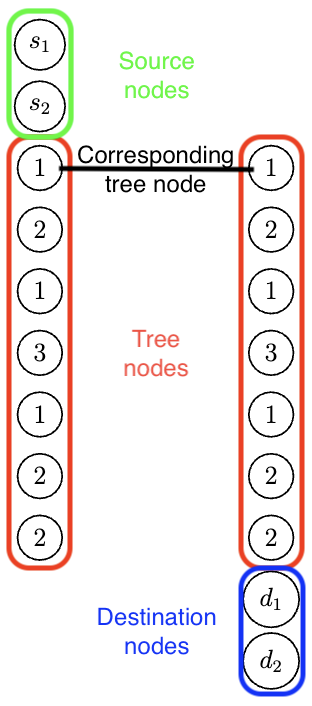
\includegraphics[width=0.3\textwidth]{Immagini/bipartite_keys_part.png}
    \caption[Bipartite nodes structure]{Example of a bipartite graph nodes constructed from a tree with the following equivalence classes $E = \{1,2,1,3,1,2,2\}$. The nodes are ordered from top to bottom.}
    \label{fig:reduction_example_parts}
\end{figure}

\begin{definition}[Bipartite graph properties]
    The resulting bipartite graph $G$ will have $2t + 2p$ nodes and $O(t (p + 1) + p^2 + tp)$ edges, where the $O(t (p + 1))$ edges come from the tree nodes, the $O(p^2)$ edges come from the sources since each source node is connected to $p$ nodes, and the $O(tp)$ edges come from the destination nodes since in the worst case we have $t$ distinct equivalence class and so all the nodes are connected to the destination nodes. The weight of the edges will be $0$ or $1$.
\end{definition}

Let's see a small example for each case, consider $p=2$. In Figure \ref{fig:reduction_small_examples}-(a) there is an example for the sources' edges, as stated before, for each source $p$ nodes with weight $1$ are created and connected to the first $p$ nodes with distinct equivalence class in $V_2$.

In Figure \ref{fig:reduction_small_examples}-(b) there is an example for the tree nodes' edges, for each node in the tree $T$ edges with weight $1$ are created and connected to the first $p$ nodes with distinct equivalence class in $V_2$ after the corresponding node in $V_2$ (coming after the node itself in the ordering), and edges with weight $0$ are created and connected to the first node with the same class in $V_2$ after the corresponding node in $V_2$. As we can see from the image, we consider the first node in $V_1$ labelled $1$ that is connected to the node $2$ with weight $1$ and to the node $3$ with weight $1$, and to the second node labelled $1$ in $V_2$ with weight $0$.

Lastly, in Figure \ref{fig:reduction_small_examples}-(c) there is an example for the destination nodes' edges, we start by considering the first node in $V_1$ that is labelled $1$, it is connected to the node $2$ with weight $1$, then since there is no node with the same class in $V_2$ we connect it to the destination nodes $d_1$ and $d_2$ with weight $0$. The same is done for the second node in $V_1$ that is labelled $2$ since no nodes are coming after it in the order it is connected to the destination nodes $d_1$ and $d_2$ with weight $0$.

\begin{figure}[H]
    \centering
    \begin{tabular}{ccc}
        \begin{tikzpicture}[node distance={10mm}, thick, auto=center, main/.style = {draw, circle}]
            \node[main] (1s) {$s_1$};
            \node[main] (2s) [below of=1s] {$s_2$};
            \node[main] (3s) [below of=2s] {$1$};
            \node[main] (4s) [below of=3s] {$1$};
            \node[main] (5s) [below of=4s] {$2$};

            \node[main] (1d) [right=3cm of 3s] {$1$};
            \node[main] (2d) [below of=1d] {$1$};
            \node[main] (3d) [below of=2d] {$2$};

            \draw[red, ->] (1s) -- (1d);
            \draw[red, ->] (1s) -- (3d);
            \draw[red, ->] (2s) -- (1d);
            \draw[red, ->] (2s) -- (3d);
        \end{tikzpicture} &
        \begin{tikzpicture}[node distance={10mm}, thick, auto=center, main/.style = {draw, circle}]
            \node[main] (3s) [below of=2s] {$1$};
            \node[main] (4s) [below of=3s] {$2$};
            \node[main] (5s) [below of=4s] {$1$};
            \node[main] (6s) [below of=5s] {$3$};
            \node[main] (1d) [right=3cm of 3s] {$1$};
            \node[main] (2d) [below of=1d] {$2$};
            \node[main] (3d) [below of=2d] {$1$};
            \node[main] (4d) [below of=3d] {$3$};

            \draw[red, ->] (3s) -- (2d);
            \draw[red, ->] (3s) -- (4d);
            \draw[green, ->] (3s) -- (3d);
        \end{tikzpicture} &
        \begin{tikzpicture}[node distance={10mm}, thick, auto=center, main/.style = {draw, circle}]
            \node[main] (7s) [below of=6s] {$1$};
            \node[main] (9s) [below of=7s] {$2$};
            \node[main] (5d) [below of=4d] {$1$};
            \node[main] (6d) [below of=5d] {$2$};
            \node[main] (8d) [below of=6d] {$d_1$};
            \node[main] (9d) [below of=8d] {$d_2$};

            \draw[red, ->] (7s) -- (6d);
            \draw[green, ->] (7s) -- (8d);
            \draw[green, ->] (7s) -- (9d);
            \draw[green, ->] (9s) -- (8d);
            \draw[green, ->] (9s) -- (9d);
        \end{tikzpicture} \\
    (a) & (b) & (c) \\
    \end{tabular}
    \caption[Reduction cases examples]{Considering $p=2$ these three examples show how to connect nodes in the bipartite graph in the case of sources (a), tree nodes (b), and destinations (c).}
    \label{fig:reduction_small_examples}
\end{figure}

\subsection{Proof of correctness}
In order to prove the correctness of the reduction, it is important to start by defining the problem we want to solve.

\begin{definition}[\textsc{CHAINS-DIVISION} problem] \label{def:problem_def}
    Given a tree $T$ with $t$ nodes, and given the equivalence classes $E$ coming from the Hopcroft algorithm applied to the tree $T$, the sorted order of the nodes in $T$ according to the upward path $\pi$, and the number of chain $p \leq t$, we want to find the optimal partition of the nodes of $T$ into $p$ chains with $p \leq t$ such that the run length encoding of each chain is minimized.
\end{definition}

Let's give a formal definition of run length encoding.
\begin{definition}[Run length encoding]
    Given a sequence $S = \{s_1, s_2, \dots, s_n\}$, the run length encoding of $S$ is the sequence $R = \{r_1, r_2, \dots, r_m\}$ where $r_i$ is the number of times the element $s_i$ is repeated in $S$. It allows us to represent the sequence $S$ in a more compact way.
\end{definition}

So, we aim to divide the nodes of the tree into $p$ chains such that the run length encoding of the chains is minimized meaning that we want to minimize the number of distinct equivalence classes in each chain. Follows the definition of chain.

\begin{definition}[Chains] \label{def:chains}
    Given a tree $T$ with $t$ nodes and $p$ chains, a chain $C$ is a sequence of nodes $C = \{c_1, c_2, \dots, c_m\}$ such that $c_i$ is a node of $T$ for $i = 1, 2, \dots, m$ and $m \leq t$. Also, Each node of $T$ is in exactly one chain and the nodes of the chain are ordered according to the upward path $\pi$ of the tree.
\end{definition}

Let's start by stating the following lemma.

\begin{lemma} \label{lemma:all_destinations}
    Exactly $|E|$ nodes of the tree $T$ of the set $V_1$ are connected each to all the destination nodes $d_i \in V_2 \quad \forall i = 1, 2, \dots, p$ with weight $0$. Where $E$ is the set of equivalence classes of the nodes of $T$ coming from the Hopcroft algorithm applied to the tree $T$.
\end{lemma}

\begin{proof}
    Since the destination nodes $d_i \in V_2$ are connected to the nodes of the tree $T$ with weight $0$ only if there is no other node with the same class in $V_2$ coming after the node in the ordering, then for sure there are $|E|$ nodes of the tree $T$ in $V_1$ that have no other node with the same class in $V_2$ coming after the node in the ordering.
\end{proof}

\begin{lemma} \label{lemma:optimal_cost}
    The optimal solution of the \textit{CHAINS-DIVISION} problem for an instance $\mathcal I$ for a tree $T$ is always greater or equal to the number of equivalence classes coming from the Hopcroft algorithm applied to the tree $T$.
\end{lemma}

\begin{proof}
    Since we aim to minimize the run length encoding of the chains, and the minimum cost of a chain is $1$, then the optimal cost of the \textit{CHAINS-DIVISION} problem for the tree $T$ is always greater or equal to the number of equivalence classes since if we dispose them in $|E|$ chains we will have a cost of $|E|$ since each chain contains only nodes with the same class, and if we dispose them in $p < |E|$ chains we will have a cost greater or equal to $|E|$ since we will have to put at least two nodes with the same class into one chain or more than one.
\end{proof}

\begin{lemma} \label{lemma:p_less_than_E}
    The solutions for the \textit{CHAINS-DIVISION} problem for the instances where the number $p$ of chains is greater than $|E|$ are not better than the solutions for the instances where $p \leq |E|$.
\end{lemma}

\begin{proof}
    The proof comes directly from lemma \ref{lemma:optimal_cost}.
\end{proof}

\begin{lemma} \label{lemma:matching_existence}
    A perfect matching for a bipartite graph $G$ constructed as stated in Definition \ref{def:bip_construction} exist for each possible instance of the \textit{CHAINS-DIVISION} problem.
\end{lemma}

\begin{proof}
    The proof comes from the construction of the bipartite graph $G$ and from theorem \ref{thm:perfect_matching_existence}. We are going to proof that the bipartite graph $G$ constructed as stated in Definition \ref{def:bip_construction} has a Tutte matrix (definition \ref{def:tutte_matrix}) with determinant different from $0$ and so a perfect matching for $G$ exists.

    We know that a $n \times n$ matrix $M$ has $Det(M) \neq 0$ if and only if it has full rank ($rank(M) = n$), or equivalently if it has $n$ linearly independent rows or columns. We can see that the bipartite graph $G$ has $2t + 2p$ nodes and $O(t (p + 1) + p^2 + tp)$ edges, and so the Tutte matrix of $G$ will have $2t + 2p$ rows and $2t + 2p$ columns. The columns of $M$ are all independent since each node of $G$ in $V_1$ is connected only to nodes in $V_2$ that are greater than $u$ in the ordering. Also each node is connected to at least one node in $V_2$ and at most $p + 1$ distinct nodes with distinct class in $V_2$. Those conditions on the edges are sufficient to get a full rank matrix and so a perfect matching for $G$ exists.
\end{proof}

In figure \ref{fig:tutte_matrix_ex} the Tutte matrix for the bipartite graph in Figure \ref{fig:reduction_example}-(a) is shown.

\begin{figure}
    \centering
    \[
    \begin{array}{c|ccccccccc}
            & \text{1} & \text{2} & \text{1} & \text{3} & \text{1} & \text{2} & \text{2} & \text{$d_1$} & \text{$d_2$} \\
        \hline
        \text{$s_1$} & 1 & 1 & 0 & 0 & 0 & 0 & 0 & 0 & 0 \\
        \text{$s_2$} & 1 & 1 & 0 & 0 & 0 & 0 & 0 & 0 & 0 \\
        \text{1}   & 0 & 1 & 1 & 1 & 0 & 0 & 0 & 0 & 0 \\
        \text{2}   & 0 & 0 & 1 & 1 & 0 & 1 & 0 & 0 & 0 \\
        \text{1}   & 0 & 0 & 0 & 1 & 1 & 1 & 0 & 0 & 0 \\
        \text{3}   & 0 & 0 & 0 & 0 & 1 & 1 & 0 & 1 & 1 \\
        \text{1}   & 0 & 0 & 0 & 0 & 0 & 1 & 0 & 1 & 1 \\
        \text{2}   & 0 & 0 & 0 & 0 & 0 & 0 & 1 & 0 & 0 \\
        \text{2}   & 0 & 0 & 0 & 0 & 0 & 0 & 0 & 1 & 1 \\
    \end{array}
    \]
    \caption[Tutte matrix example]{Example of a Tutte matrix for a bipartite graph in figure \ref{fig:reduction_example}-(a). As we can see the matrix has full rank and so a perfect matching exists.}
    \label{fig:tutte_matrix_ex}
\end{figure}

\begin{lemma} \label{lemma:greater_nodes}
    Given a bipartite graph $G$ constructed as stated in Definition \ref{def:bip_construction} from a tree $T$, for each node $u \in V_1$ coming from the nodes of $T$ it is impossible for $u$ to be connected to node $v \in V_2$ coming from the nodes of $T$ such as $v < u$ in the order of the nodes of the tree $T$.
\end{lemma}

\begin{proof}
    The proof comes from the construction of $G$ where the nodes of $V_1$ are always connected to the nodes of $V_2$ coming after them in the ordering of the nodes of the tree $T$.
\end{proof}

Now we can prove the correctness of the reduction.

\begin{theorem}
    An optimal solution of an instance $\mathcal I$ with $p \leq |E|$ of the problem defined in Definition \ref{def:problem_def} is equivalent to an optimal solution of the Minimum Weight Perfect Bipartite Matching for the instance $r(\mathcal I)$ where $r: \mathcal{I}_{CHAINS-DIVISION} \rightarrow \mathcal{I}_{MWPBM}$ is the reduction function that maps an instance of the problem defined in Definition \ref{def:problem_def} to an instance of the Minimum Weight Perfect Bipartite Matching problem defined in Definition \ref{def:mwpbm} constructed as stated in Definition \ref{def:bip_construction}.
\end{theorem}

\begin{proof}
    Let $p \leq t$ be the number of chains we want to partition the nodes of a given tree $T$ into. Let $E$ be the set of equivalence classes of the nodes of $T$, from lemma \ref{lemma:p_less_than_E} we consider that $p \leq |E|$. We can construct a bipartite graph $G = (V, E)$ such that vertices are divided in two disjoint sets $V = V_1 \cup V_2$ as stated in Definition \ref{def:bip_construction}. We will show that the optimal solution of the Minimum Weight Perfect Bipartite Matching problem for the graph $G$ is equivalent to the optimal solution of the \textsc{CHAINS-DIVISION} problem for the tree $T$.

    From definition \ref{def:bip_construction} we know that $V_1$ contains $t + p$ nodes including $s_1, s_2, \dots, s_p$ and the $t$ elements of $E$ ordered, and $V_2$ contains $t + p$ nodes including the $t$ elements of $E$ ordered and $d_1, d_2, \dots, d_p$.

    The source nodes are necessary to distinguish the chains, by starting from each source node we can follow the edges of the nodes and reach the destination nodes in order to retrieve the nodes of a chain. The source nodes are all connected to the first $p$ nodes with distinct equivalence class in $V_2$ with weight $1$ since each chains has at least one node and a minimum cost of $1$.

    The destination nodes are necessary to close the chains, by connecting the nodes of the tree to the destination nodes we can ensure that the chains are closed and allows to get a perfect matching otherwise we would have $|V_1| > |V_2|$ and so we would have unmatched nodes. From lemma \ref{lemma:all_destinations} we know that exactly $|E|$ nodes of the tree $T$ in $V_1$ are connected to all the destination nodes $d_i \in V_2 \quad \forall i = 1, 2, \dots, p$ with weight $0$. This is done in order to ensure that the chains are closed and that the nodes of the tree are connected to the destination nodes in order to have a perfect matching. The weight of the edges is $0$ since if we conclude a chain no additional cost is needed.

    We know from definition \ref{def:chains} that the order of the nodes of each chain must follow the order given by the upward path $\pi$ of each node in the tree $T$. This is ensured by lemma \ref{lemma:greater_nodes} that states that it is impossible for a node $u \in V_1$ coming from the nodes of $T$ to be connected to a node $v \in V_2$ coming from the nodes of $T$ such as $v < u$ in the order of the nodes of the tree $T$. This is done in order to ensure that the nodes are connected in the right order.

    Given the construction of the bipartite graph $G$ we can see that the optimal solution of the Minimum Weight Perfect Bipartite Matching problem for the graph $G$ is equivalent to the optimal solution of the \textsc{CHAINS-DIVISION} problem for the tree $T$ since the chains are closed and the nodes are connected in the right order. The weight of the edges $0$ allow the problem to chain subsequent nodes with the same class without adding additional cost. Also from the definition of matching (\ref{def:matching}) no node of $G$ is exposed and so the matching is perfect as proved in lemma \ref{lemma:matching_existence}. The fact that each node in $V_1$ is connected to at least $p$ edges allow the problem to compare all the possible chains and so to find the optimal solution.
\end{proof}

\subsection{Full example}
Consider The example in Figure \ref{fig:reduction_example} where we have a tree $T$ with $t=7$ nodes, $p = 2$ chains and the equivalence classes $E = \{1,2,1,3,1,2,2\}$ sorted accordingly to the upward path $\pi$ of each node of the tree. We can construct the two distinct sets $V_1$ and $V_2$ of the bipartite graph $G$ as follows: $V_1 = \{s_1, s_2, 1,2,1,3,1,2,2\}$ and $V_2 = \{1,2,1,3,1,2,2, d_1, d_2\}$. The edges of the graph $G$ will be constructed as stated in Definition \ref{def:bip_construction}. In Figure \ref{fig:reduction_example}-(a) we have the resulting bipartite graph, and in Figure \ref{fig:reduction_example}-(b) we have one of the possible minimum perfect matchings for the graph in (a) having weight $4$. A the end we can see that the optimal partition of the nodes of the tree $T$ is $C_1 = \{1,1,1,2,2\}$ and $C_2 = \{2,3\}$ with a total cost of $4$, this can be obtained starting from the sources and by following the edges of the nodes, jumping to the corresponding node in $V_1$ and following the edges again until we reach the destination nodes.

\begin{figure}[H]
    \centering
    \begin{tabular}{cc}
        \begin{tikzpicture}[node distance={10mm}, thick, auto=center, main/.style = {draw, circle}]
            \node[main] (1s) {$s_1$};
            \node[main] (2s) [below of=1s] {$s_2$};
            \node[main] (3s) [below of=2s] {$1$};
            \node[main] (4s) [below of=3s] {$2$};
            \node[main] (5s) [below of=4s] {$1$};
            \node[main] (6s) [below of=5s] {$3$};
            \node[main] (7s) [below of=6s] {$1$};
            \node[main] (8s) [below of=7s] {$2$};
            \node[main] (9s) [below of=8s] {$2$};
            \node[main] (1d) [right=3cm of 3s] {$1$};
            \node[main] (2d) [below of=1d] {$2$};
            \node[main] (3d) [below of=2d] {$1$};
            \node[main] (4d) [below of=3d] {$3$};
            \node[main] (5d) [below of=4d] {$1$};
            \node[main] (6d) [below of=5d] {$2$};
            \node[main] (7d) [below of=6d] {$2$};
            \node[main] (8d) [below of=7d] {$d_1$};
            \node[main] (9d) [below of=8d] {$d_2$};

            \draw[red, ->] (1s) -- (1d);
            \draw[red, ->] (1s) -- (2d);
            \draw[red, ->] (2s) -- (1d);
            \draw[red, ->] (2s) -- (2d);
            \draw[red, ->] (3s) -- (2d);
            \draw[red, ->] (3s) -- (4d);
            \draw[green, ->] (3s) -- (3d);
            \draw[red, ->] (4s) -- (3d);
            \draw[red, ->] (4s) -- (4d);
            \draw[green, ->] (4s) -- (6d);
            \draw[red, ->] (5s) -- (4d);
            \draw[green, ->] (5s) -- (5d);
            \draw[red, ->] (5s) -- (6d);
            \draw[red, ->] (6s) -- (5d);
            \draw[red, ->] (6s) -- (6d);
            \draw[green, ->] (6s) -- (8d);
            \draw[green, ->] (6s) -- (9d);
            \draw[red, ->] (7s) -- (6d);
            \draw[green, ->] (7s) -- (8d);
            \draw[green, ->] (7s) -- (9d);
            \draw[green, ->] (8s) -- (7d);
            \draw[green, ->] (9s) -- (8d);
            \draw[green, ->] (9s) -- (9d);
        \end{tikzpicture} &
        \begin{tikzpicture}[node distance={10mm}, thick, auto=center, main/.style = {draw, circle}]
            \node[main] (1s) {$s_1$};
            \node[main] (2s) [below of=1s] {$s_2$};
            \node[main] (3s) [below of=2s] {$1$};
            \node[main] (4s) [below of=3s] {$2$};
            \node[main] (5s) [below of=4s] {$1$};
            \node[main] (6s) [below of=5s] {$3$};
            \node[main] (7s) [below of=6s] {$1$};
            \node[main] (8s) [below of=7s] {$2$};
            \node[main] (9s) [below of=8s] {$2$};
            \node[main] (1d) [right=3cm of 3s] {$1$};
            \node[main] (2d) [below of=1d] {$2$};
            \node[main] (3d) [below of=2d] {$1$};
            \node[main] (4d) [below of=3d] {$3$};
            \node[main] (5d) [below of=4d] {$1$};
            \node[main] (6d) [below of=5d] {$2$};
            \node[main] (7d) [below of=6d] {$2$};
            \node[main] (8d) [below of=7d] {$d_1$};
            \node[main] (9d) [below of=8d] {$d_2$};

            \draw[red, ->] (1s) -- (1d);
            \draw[red, ->] (2s) -- (2d);
            \draw[green, ->] (3s) -- (3d);
            \draw[red, ->] (4s) -- (4d);
            \draw[green, ->] (5s) -- (5d);
            \draw[green, ->] (6s) -- (8d);
            \draw[red, ->] (7s) -- (6d);
            \draw[green, ->] (8s) -- (7d);
            \draw[green, ->] (9s) -- (9d);
        \end{tikzpicture} \\
    (a) & (b) \\
    \end{tabular}
    \caption[Reduction full example]{Example of a reduction for the sorted nodes' equivalency classes $E = \{1,2,1,3,1,2,2\}$. In (a), we have the resulting bipartite graph constructed from $E$. In (b), we have the resulting perfect matching for the graph in (a) having weight $4$. Green edges weigh $0$, while red edges weigh $1$.}
    \label{fig:reduction_example}
\end{figure}

\section{Heuristics and Improvements}
Some changes can be made to the reduction in order to optimize it and to reduce the number of edges in the bipartite graph. Here are some of the improvements that can be made.

\begin{itemize}
    \item \textbf{Sources' edges optimization}:
    \begin{lemma} \label{lemma:sources_optimization}
        The sources' edges can be optimized by connecting each source only to the smaller node (considering the order of the nodes) in $V_2$ coming from the tree $T$ that is not connected to any other source.
    \end{lemma}

    \begin{proof}
        Since the source nodes are needed to distinguish the chains as starting points, we need that each source is connected to at least one node in $V_2$ coming from the tree $T$. Having the sources connected to the first $p$ nodes with distinct equivalence class in $V_2$ is not necessary since allows us just to invert the chains starting from each source and so it is redundant. We can connect each source to the smaller node in $V_2$ coming from the tree $T$ that is not connected to any other source since we need to connect each source to at least one node in $V_2$ coming from the tree $T$ and this will allow us to distinguish the chains.
    \end{proof}

    This will reduce the number of edges coming from the sources from $O(p^2)$ to $O(p)$. In Figure \ref{fig:heuristics_example}-(a) the removed edges are shown in green.
    \item \textbf{Tree nodes' edges optimization 1}:
    \begin{lemma} \label{lemma:tree_optimization_1}
        The tree nodes' edges can be optimized by removing the edges of tree nodes that are connected to nodes in $V_2$ already linked to a source node in $V_1$.
    \end{lemma}

    \begin{proof}
        From definition \ref{def:matching} we know that a matching $M \in E$ is a collection of edges such that every vertex of $V$ is incident to at most one edge of $M$. In other words, a matching is a set of edges such that no two edges share a common vertex. Given that, in all the solutions to the problem all sources will be connected to exactly one node in $V_2$ coming from the tree $T$ and so we can remove the edges of the tree nodes that are connected to nodes in $V_2$ already linked to a source node in $V_1$ since they will not be part of the final matching.
    \end{proof}

    This will reduce the number of edges by a factor of $O(p - 1)$. In Figure \ref{fig:heuristics_example}-(a) the removed edges are shown in blue.

    \item \textbf{Tree nodes' edges optimization 2}:
    \begin{lemma} \label{lemma:tree_optimization_2}
        The tree nodes' edges can be optimized by removing the edges with weight $1$ starting from a node $u \in V_1$ to a node $v \in V_2$ if the node $u$ has another edge with weight $0$ connected to a node $z \in V_2$ such that $z < v$ in the ordering of the nodes.
    \end{lemma}

    \begin{proof}
        To proof the lemma since every time we have an edge with weight $0$ between two nodes of $V_1$ and $V_2$ it means that those two nodes have the same equivalence class and so there is no need to add additional cost trying to connect that node to nodes with different classes coming after in the ordering, as that would only increase the cost without providing any benefit to the solution. Also, we know that connecting nodes with the same class is always the best choice for optimizing the run length encoding of each chain.
    \end{proof}

    In Figure \ref{fig:heuristics_example}-(a) the removed edges are shown in red.
\end{itemize}

In figure \ref{fig:heuristics_example}-(b) we can see the resulting bipartite graph for the example shown in previous section after the optimizations.

\begin{figure}[H]
    \centering
    \begin{tabular}{cc}
        \begin{tikzpicture}[node distance={10mm}, thick, auto=center, main/.style = {draw, circle}]
            \node[main] (1s) {$s_1$};
            \node[main] (2s) [below of=1s] {$s_2$};
            \node[main] (3s) [below of=2s] {$1$};
            \node[main] (4s) [below of=3s] {$2$};
            \node[main] (5s) [below of=4s] {$1$};
            \node[main] (6s) [below of=5s] {$3$};
            \node[main] (7s) [below of=6s] {$1$};
            \node[main] (8s) [below of=7s] {$2$};
            \node[main] (9s) [below of=8s] {$2$};
            \node[main] (1d) [right=3cm of 3s] {$1$};
            \node[main] (2d) [below of=1d] {$2$};
            \node[main] (3d) [below of=2d] {$1$};
            \node[main] (4d) [below of=3d] {$3$};
            \node[main] (5d) [below of=4d] {$1$};
            \node[main] (6d) [below of=5d] {$2$};
            \node[main] (7d) [below of=6d] {$2$};
            \node[main] (8d) [below of=7d] {$d_1$};
            \node[main] (9d) [below of=8d] {$d_2$};

            \draw[black, dashed, ->] (1s) -- (1d);
            \draw[green, dashed, ->] (1s) -- (2d);
            \draw[green, dashed, ->] (2s) -- (1d);
            \draw[black, dashed, ->] (2s) -- (2d);
            \draw[blue, dashed, ->] (3s) -- (2d);
            \draw[red, dashed, ->] (3s) -- (4d);
            \draw[black, ->] (3s) -- (3d);
            \draw[black, dashed, ->] (4s) -- (3d);
            \draw[black, dashed, ->] (4s) -- (4d);
            \draw[black, ->] (4s) -- (6d);
            \draw[black, dashed, ->] (5s) -- (4d);
            \draw[black, ->] (5s) -- (5d);
            \draw[red, dashed, ->] (5s) -- (6d);
            \draw[black, dashed, ->] (6s) -- (5d);
            \draw[black, dashed, ->] (6s) -- (6d);
            \draw[black, ->] (6s) -- (8d);
            \draw[black, ->] (6s) -- (9d);
            \draw[black, dashed, ->] (7s) -- (6d);
            \draw[black, ->] (7s) -- (8d);
            \draw[black, ->] (7s) -- (9d);
            \draw[black, ->] (8s) -- (7d);
            \draw[black, ->] (9s) -- (8d);
            \draw[black, ->] (9s) -- (9d);
        \end{tikzpicture} &
        \begin{tikzpicture}[node distance={10mm}, thick, auto=center, main/.style = {draw, circle}]
            \node[main] (1s) {$s_1$};
            \node[main] (2s) [below of=1s] {$s_2$};
            \node[main] (3s) [below of=2s] {$1$};
            \node[main] (4s) [below of=3s] {$2$};
            \node[main] (5s) [below of=4s] {$1$};
            \node[main] (6s) [below of=5s] {$3$};
            \node[main] (7s) [below of=6s] {$1$};
            \node[main] (8s) [below of=7s] {$2$};
            \node[main] (9s) [below of=8s] {$2$};
            \node[main] (1d) [right=3cm of 3s] {$1$};
            \node[main] (2d) [below of=1d] {$2$};
            \node[main] (3d) [below of=2d] {$1$};
            \node[main] (4d) [below of=3d] {$3$};
            \node[main] (5d) [below of=4d] {$1$};
            \node[main] (6d) [below of=5d] {$2$};
            \node[main] (7d) [below of=6d] {$2$};
            \node[main] (8d) [below of=7d] {$d_1$};
            \node[main] (9d) [below of=8d] {$d_2$};

            \draw[black, dashed, ->] (1s) -- (1d);
            \draw[black, dashed, ->] (2s) -- (2d);
            \draw[black, ->] (3s) -- (3d);
            \draw[black, dashed, ->] (4s) -- (3d);
            \draw[black, dashed, ->] (4s) -- (4d);
            \draw[black, ->] (4s) -- (6d);
            \draw[black, dashed, ->] (5s) -- (4d);
            \draw[black, ->] (5s) -- (5d);
            \draw[black, dashed, ->] (6s) -- (5d);
            \draw[black, dashed, ->] (6s) -- (6d);
            \draw[black, ->] (6s) -- (8d);
            \draw[black, ->] (6s) -- (9d);
            \draw[black, dashed, ->] (7s) -- (6d);
            \draw[black, ->] (7s) -- (8d);
            \draw[black, ->] (7s) -- (9d);
            \draw[black, ->] (8s) -- (7d);
            \draw[black, ->] (9s) -- (8d);
            \draw[black, ->] (9s) -- (9d);
        \end{tikzpicture} \\
    (a) & (b) \\
    \end{tabular}
    \caption[Reduction heuristics example]{Example of a reduction for the sorted nodes' equivalency classes $E = \{1,2,1,3,1,2,2\}$ applying also the heuristics showed. In (a), the edges removed are shown in green for lemma \ref{lemma:sources_optimization}, blue for lemma \ref{lemma:tree_optimization_1}, and red for lemma \ref{lemma:tree_optimization_2}. In (b), we have the resulting bipartite graph after the heuristics applied. Dashed edges weigh $1$, while solid edges weigh $0$.}
    \label{fig:heuristics_example}
\end{figure}

\section{Moving to Maximum weight perfect bipartite matching}
In this section, we will discuss how to slightly modify the reduction process to move from a minimum weight perfect bipartite matching problem to a maximum weight perfect bipartite matching problem. This will be helpful in solving the problem more efficiently by using some known algorithms to solve the maximum weight perfect bipartite matching problem.

\begin{theorem}
    An optimal solution of an instance $\mathcal I$ with $p \leq |E|$ of the \textsc{CHAINS-DIVISION} problem is equivalent to an optimal solution of the Maximum Weight Perfect Bipartite Matching for the instance $r(\mathcal I)$ where $r: \mathcal{I}_{CHAINS-DIVISION} \rightarrow \mathcal{I}_{MWPBM}$ is the reduction function that maps an instance of the CHAINS-DIVISION problem to an instance of the Maximum Weight Perfect Bipartite Matching problem constructed as stated in Definition \ref{def:bip_construction} but with inverted weights (weight $0$ becomes $1$ and weight $1$ becomes $0$).
\end{theorem}

\begin{proof}
    Let $M$ be a perfect matching in the bipartite graph $G$ constructed as stated in Definition \ref{def:bip_construction}. Let $w(M)$ be the sum of the weights of the edges in the matching $M$. From the previous theorem, we know that the optimal solution of the \textsc{CHAINS-DIVISION} problem is equivalent to finding a perfect matching $M$ in $G$ that minimizes $w(M)$.

    Let $G'$ be a bipartite graph constructed as $G$ but with inverted weights (weight $0$ becomes $1$ and weight $1$ becomes $0$). Let $M'$ be a perfect matching in $G'$ and let $w'(M')$ be the sum of the weights of the edges in the matching $M'$. Let $k$ be the number of edges in the matching.

    We can see that for any matching $M$ in $G$:
    \[ w'(M) = k - w(M) \]

    This means that maximizing $w'(M)$ is equivalent to minimizing $w(M)$. Therefore, finding the maximum weight perfect matching in $G'$ is equivalent to finding the minimum weight perfect matching in $G$, which in turn is equivalent to finding the optimal solution of the \textsc{CHAINS-DIVISION} problem.
\end{proof}
